% Portfolio for Muhamad Andung Muntaha
% Styled to match the accompanying resume template
% Base template (c) 2002-2011 Boedicker/Grant/Johnston/Clark, CC BY-NC-SA 2.5

\documentclass[letterpaper,10pt]{article}
\newlength{\outerbordwidth}
\pagestyle{empty}
\raggedbottom
\raggedright
\usepackage[svgnames]{xcolor}
\usepackage{framed}
\usepackage{tocloft}
\usepackage{etoolbox}
\usepackage{graphicx}
\usepackage{tabularx}
\usepackage{hyperref}
\robustify\cftdotfill

%-----------------------------------------------------------
\setlength{\outerbordwidth}{3pt}
\definecolor{shadecolor}{gray}{0.75}
\definecolor{shadecolorB}{gray}{0.93}

%-----------------------------------------------------------
\setlength{\evensidemargin}{-0.25in}
\setlength{\headheight}{-0.25in}
\setlength{\headsep}{0in}
\setlength{\oddsidemargin}{-0.25in}
\setlength{\paperheight}{12in}
\setlength{\paperwidth}{9in}
\setlength{\tabcolsep}{0in}
\setlength{\textheight}{10.7in}
\setlength{\textwidth}{7.4in}
\setlength{\topmargin}{-0.3in}
\setlength{\topskip}{0in}
\setlength{\voffset}{0.1in}

%-----------------------------------------------------------
\newcommand{\resheading}[1]{\vspace{10pt}
  \parbox{\textwidth}{\setlength{\FrameSep}{\outerbordwidth}
    \begin{shaded}
\setlength{\fboxsep}{0pt}\framebox[\textwidth][l]{\setlength{\fboxsep}{3pt}\fcolorbox{shadecolorB}{shadecolorB}{\textbf{\sffamily{\mbox{~}\makebox[7.2in][l]{#1} \vphantom{p\^{E}}}}}}
    \end{shaded}
  }\vspace{-2pt}
}

\newcommand{\projectitem}[3]{%
  {\large\textbf{#1}} \hfill {\textit{#2}}\par
  \vspace{2pt}
  #3
}

%-----------------------------------------------------------
\begin{document}

\begin{tabular*}{7.4in}{l@{\extracolsep{\fill}}r}
  \textbf{{\Large Muhamad Andung Muntaha}} & Jakarta, Indonesia \\
  \texttt{andung07@gmail.com} & \today \\
  \texttt{+6281380260278} &
\end{tabular*}

\makebox[\linewidth]{\rule{\textwidth}{0.4pt}}\vspace{2pt}

\begin{flushleft}
\textbf{Portfolio --- Solution Architecture \& IoT Engineering.} A selection of end-to-end IoT, embedded, and edge-AI solutions architected and delivered across industrial, defense, automotive, sports-tech, and consumer domains --- spanning custom hardware, real-time firmware, cloud-scale backend systems, and mobile/web client applications. Each project demonstrates applied architecture and engineering across the full device-to-cloud stack, including embedded firmware, edge-AI inference, cloud-native backend systems, and mobile/web client applications.
\end{flushleft}\vspace{-8pt}

%%%%%%%%%%%%%%%%%%%%%%%%%%%%%%%%%%%%%%%%%%%%%%%%%%%%%%%%%%%%
\resheading{1. GymSense --- AI Fitness Tracker (XLabs, Indonesia)}
%%%%%%%%%%%%%%%%%%%%%%%%%%%%%%%%%%%%%%%%%%%%%%%%%%%%%%%%%%%%
\begin{minipage}[t]{4.5in}
\vspace{2pt}
Architected an AI-powered fitness tracking product as a flagship solution under XLabs' AI/IoT consultancy practice, demonstrating applied computer-vision and sensor-based movement analysis for real-time exercise tracking and form feedback.
\begin{itemize}
  \item Solution architecture spanning on-device inference, mobile/web client, and cloud backend
  \item Designed as a library to be integrated into third-party apps, enabling real-time exercise tracking and form feedback without requiring a dedicated device 
  \item Live at: \url{https://xlabs.id/gymsense}
\end{itemize}
\end{minipage}%
\hfill
\begin{minipage}[t]{2.5in}
\vspace{0pt}
\centering
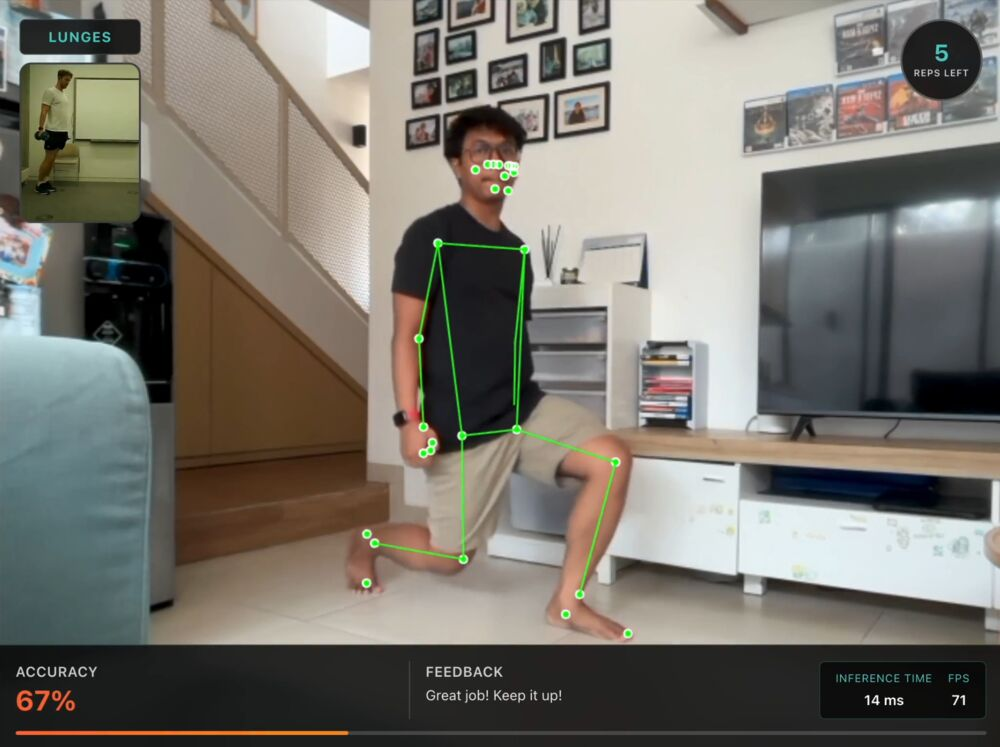
\includegraphics[width=2.5in]{image1.jpg}
\end{minipage}

\vspace{8pt}

%%%%%%%%%%%%%%%%%%%%%%%%%%%%%%%%%%%%%%%%%%%%%%%%%%%%%%%%%%%%
\resheading{2. Movaja --- AI-Coached Fitness App (XLabs, Indonesia)}
%%%%%%%%%%%%%%%%%%%%%%%%%%%%%%%%%%%%%%%%%%%%%%%%%%%%%%%%%%%%
Architected Movaja, a mobile and web fitness application combining pro-led training programs with real-time on-device AI form validation, giving users personal-trainer-level feedback without needing a gym or coach on-site. The platform spans a trainer/program marketplace, daily workout scheduling, and social leaderboard/gamification to drive engagement and retention.
\begin{itemize}
  \item End-to-end mobile and web app architecture: program marketplace, daily workout tracking, progress/XP-based leaderboard, enterprise dashboard
  \item On-device AI processing for real-time exercise form scoring, enabling offline-friendly, low-latency coaching
  \item Live at: \url{https://movaja.id}
\end{itemize}
\begin{center}
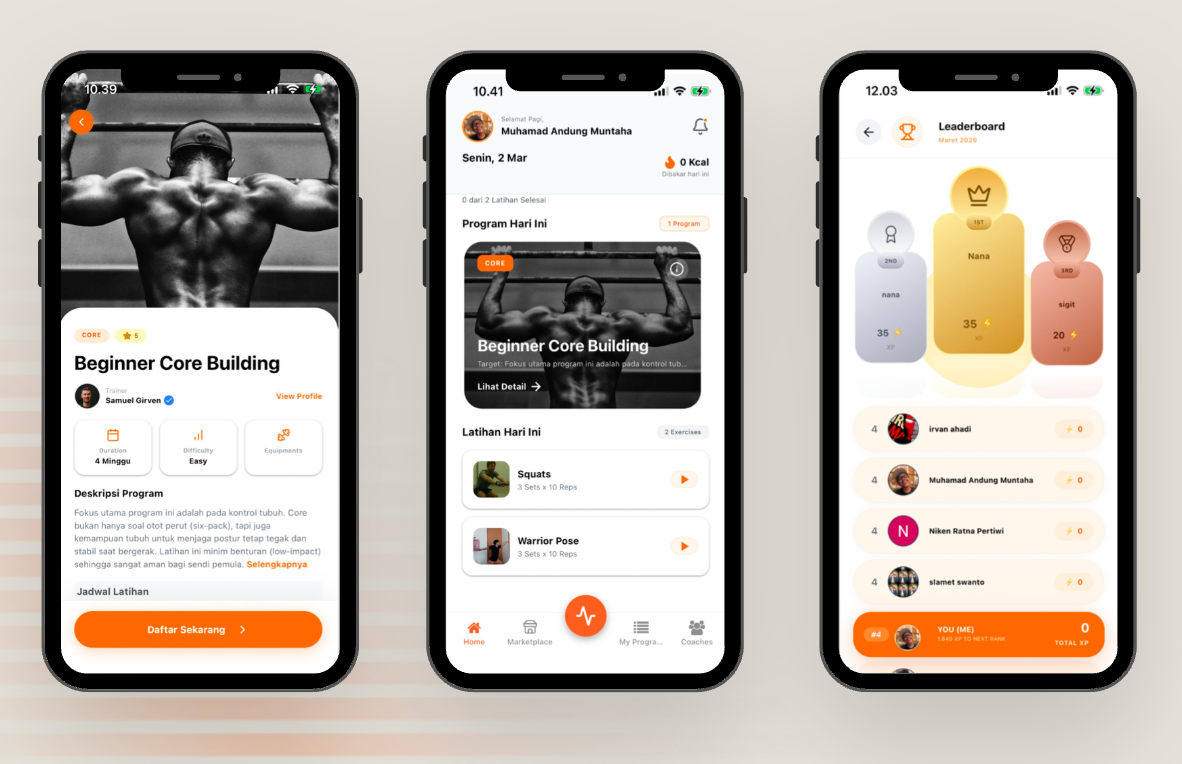
\includegraphics[width=6in]{movaja.png}
\end{center}

\vspace{8pt}

%%%%%%%%%%%%%%%%%%%%%%%%%%%%%%%%%%%%%%%%%%%%%%%%%%%%%%%%%%%%
\resheading{3. Secure Communication Device for Defense (Netra, Indonesia)}
%%%%%%%%%%%%%%%%%%%%%%%%%%%%%%%%%%%%%%%%%%%%%%%%%%%%%%%%%%%%
\begin{minipage}[t]{4.5in}
\vspace{2pt}
Led architecture and delivery of a custom embedded communication device for a defense-sector client, engineered for resilient field operation and secure data handling under mission-critical reliability requirements.
\begin{itemize}
  \item Custom hardware and embedded firmware architecture built to defense-grade reliability standards
  \item Designed secure device-to-backend communication and remote device management
  \item Coordinated cross-disciplinary hardware, firmware, and systems integration teams
\end{itemize}
\end{minipage}%
\hfill
\begin{minipage}[t]{2.5in}
\vspace{0pt}
\centering
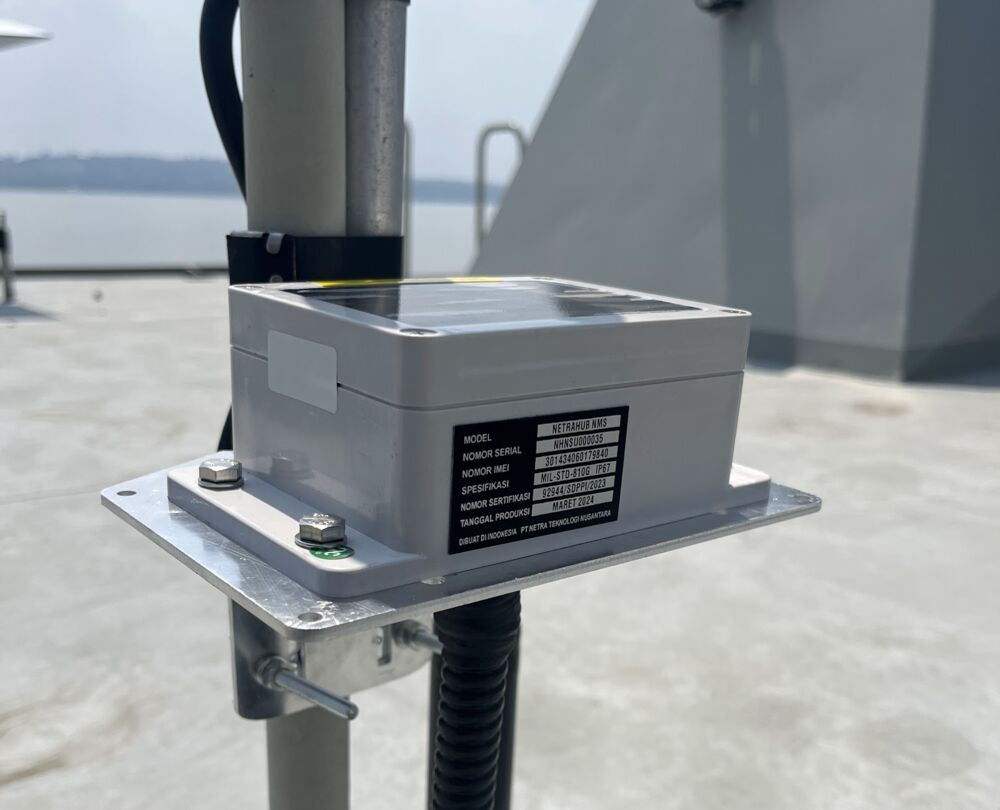
\includegraphics[width=2.4in]{image7.jpg}
\end{minipage}

\vspace{8pt}

%%%%%%%%%%%%%%%%%%%%%%%%%%%%%%%%%%%%%%%%%%%%%%%%%%%%%%%%%%%%
\resheading{4. Enterprise IoT Platform (Netra, Indonesia)}
%%%%%%%%%%%%%%%%%%%%%%%%%%%%%%%%%%%%%%%%%%%%%%%%%%%%%%%%%%%%
Architected Netra's core IoT platform, connecting distributed embedded devices deployed on custom hardware to a Kubernetes-based cloud backend --- covering device provisioning, telemetry ingestion, OTA firmware updates, and a client-facing management dashboard. Designed as the reusable architectural foundation behind multiple client engagements, prioritizing scalability, security, and maintainability across the full device-to-cloud stack.
\begin{center}
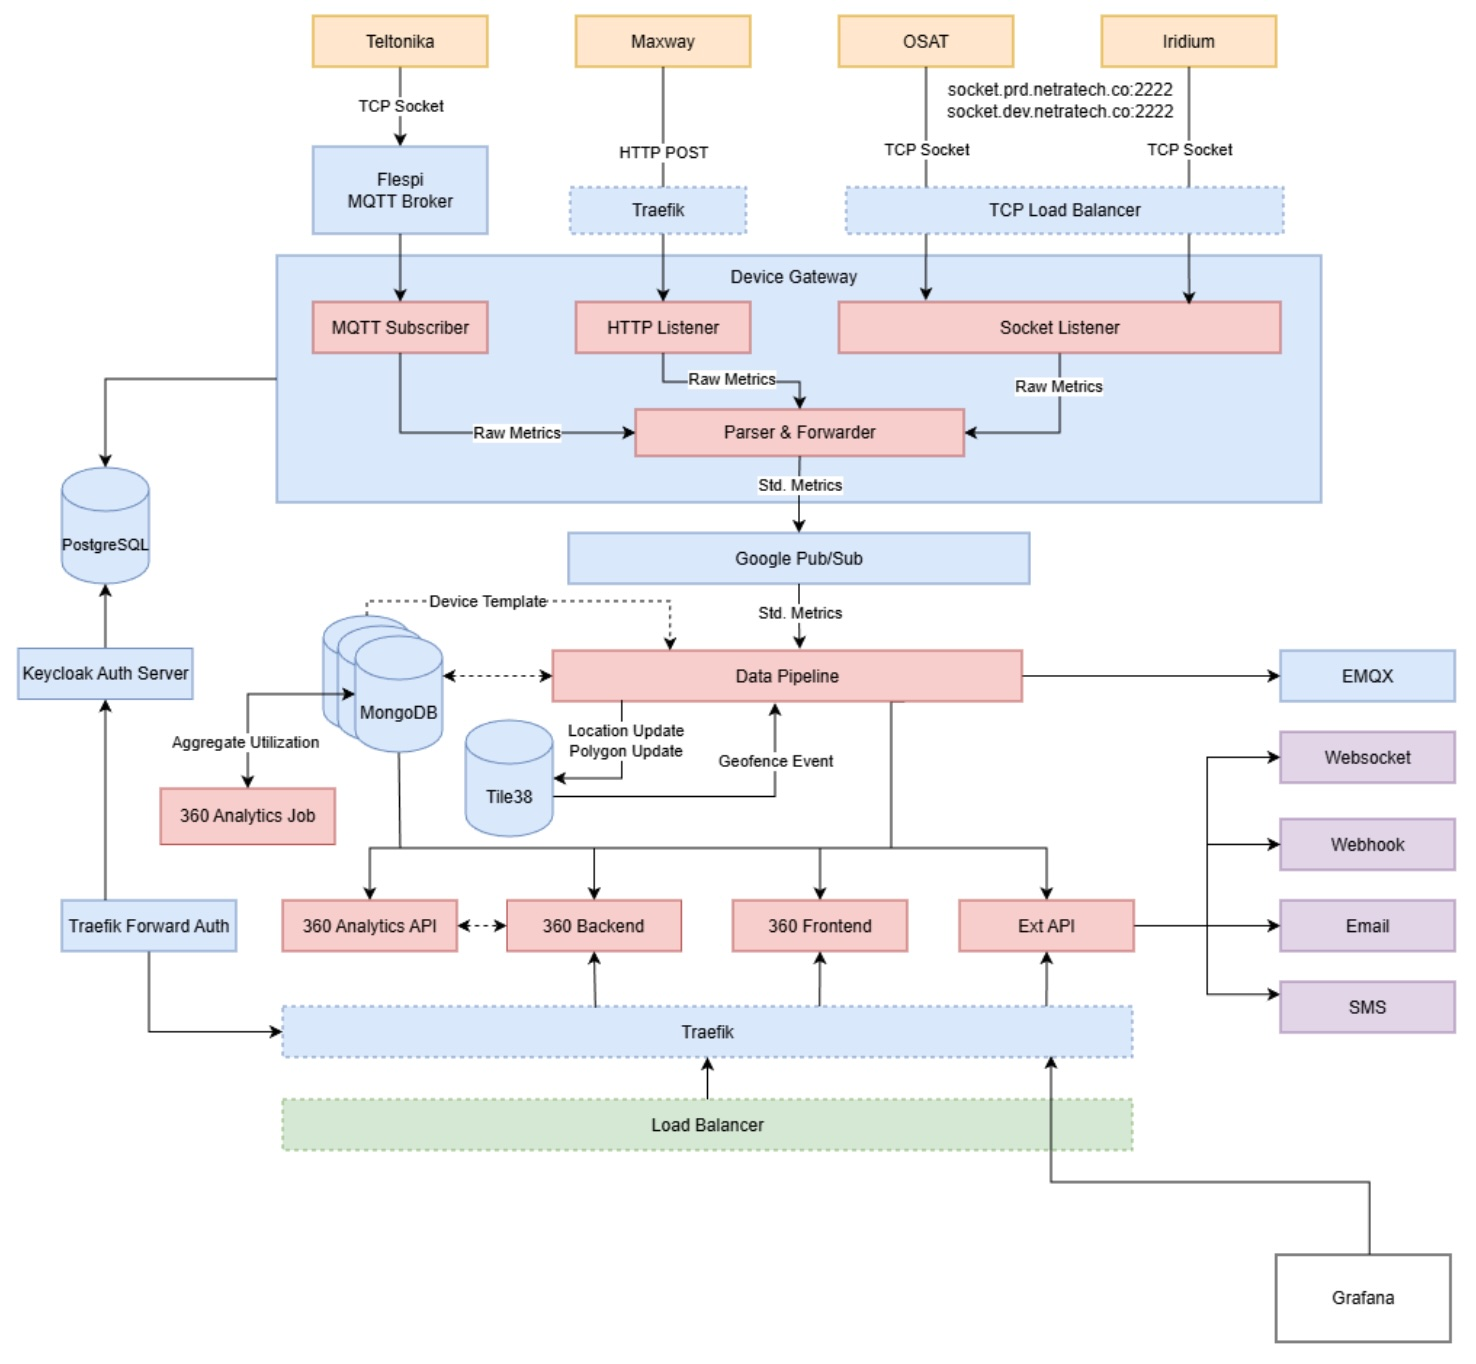
\includegraphics[width=7in]{image4.jpg}
\end{center}

\vspace{6pt}

%%%%%%%%%%%%%%%%%%%%%%%%%%%%%%%%%%%%%%%%%%%%%%%%%%%%%%%%%%%%
\resheading{5. Agora Gas Lift Optimization (SLB, Indonesia)}
%%%%%%%%%%%%%%%%%%%%%%%%%%%%%%%%%%%%%%%%%%%%%%%%%%%%%%%%%%%%
\begin{minipage}[t]{4.6in}
\vspace{2pt}
Architected and delivered Indonesia's first commercial Industrial IoT deployment: an edge-based, machine-learning-driven gas-lift optimization system built on SLB's Agora IIoT platform.
\begin{itemize}
  \item Closed-loop control architecture continuously adjusting the gas injection control valve in real time
  \item ML-based optimization algorithm deployed and executed on the edge, integrated with SCADA
  \item Delivered a measured production increase of 5 BOPD, validating the solution's commercial impact
\end{itemize}
\end{minipage}%
\hfill
\begin{minipage}[t]{2.2in}
\vspace{0pt}
\centering
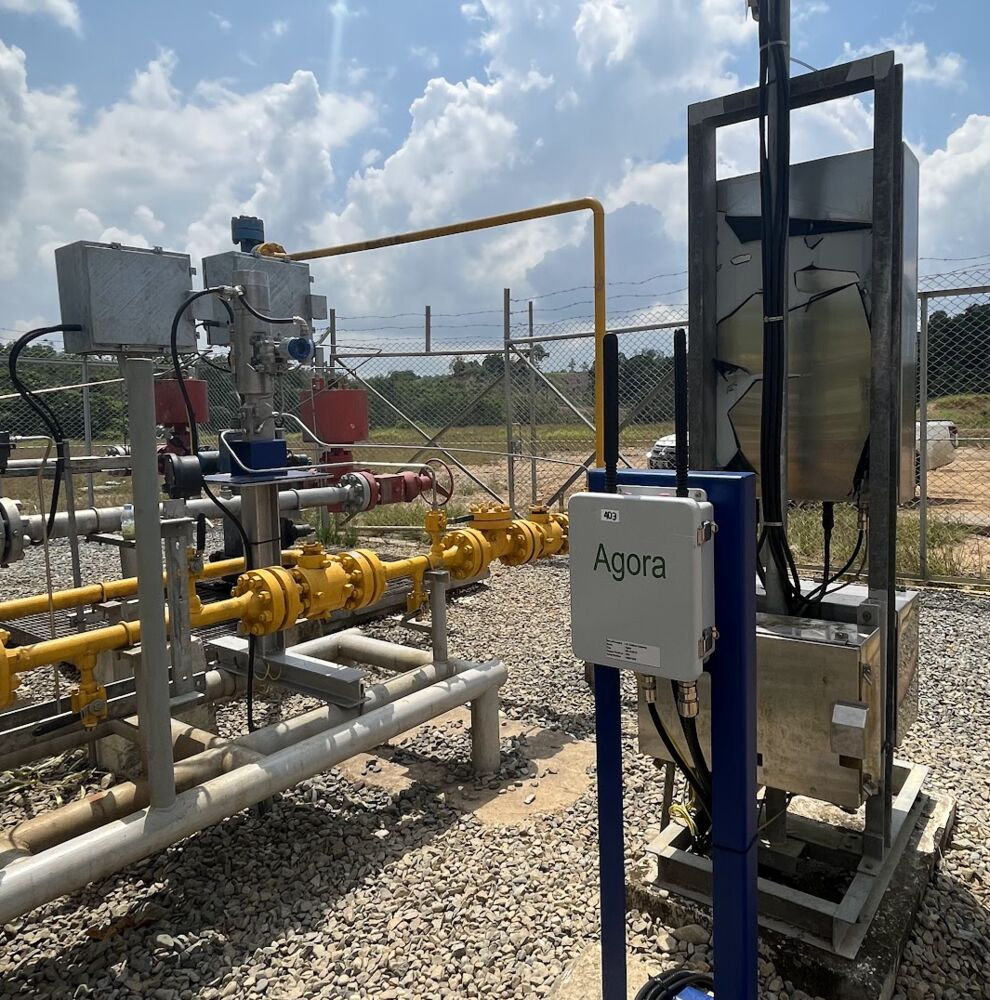
\includegraphics[width=2.1in]{image10.jpg}
\end{minipage}

\vspace{8pt}

%%%%%%%%%%%%%%%%%%%%%%%%%%%%%%%%%%%%%%%%%%%%%%%%%%%%%%%%%%%%
\resheading{6. Fleet Metering Engine (Blue Bird Group, Indonesia)}
%%%%%%%%%%%%%%%%%%%%%%%%%%%%%%%%%%%%%%%%%%%%%%%%%%%%%%%%%%%%
Architected the real-time fare metering engine embedded within Blue Bird's fleet-wide IoT device, deployed across 20,000 vehicles. Integrated directly with each vehicle's CAN bus to derive accurate distance and fare calculations from live vehicle telemetry, feeding a device-management and OTA update platform running on a Kubernetes-based backend.
\begin{center}
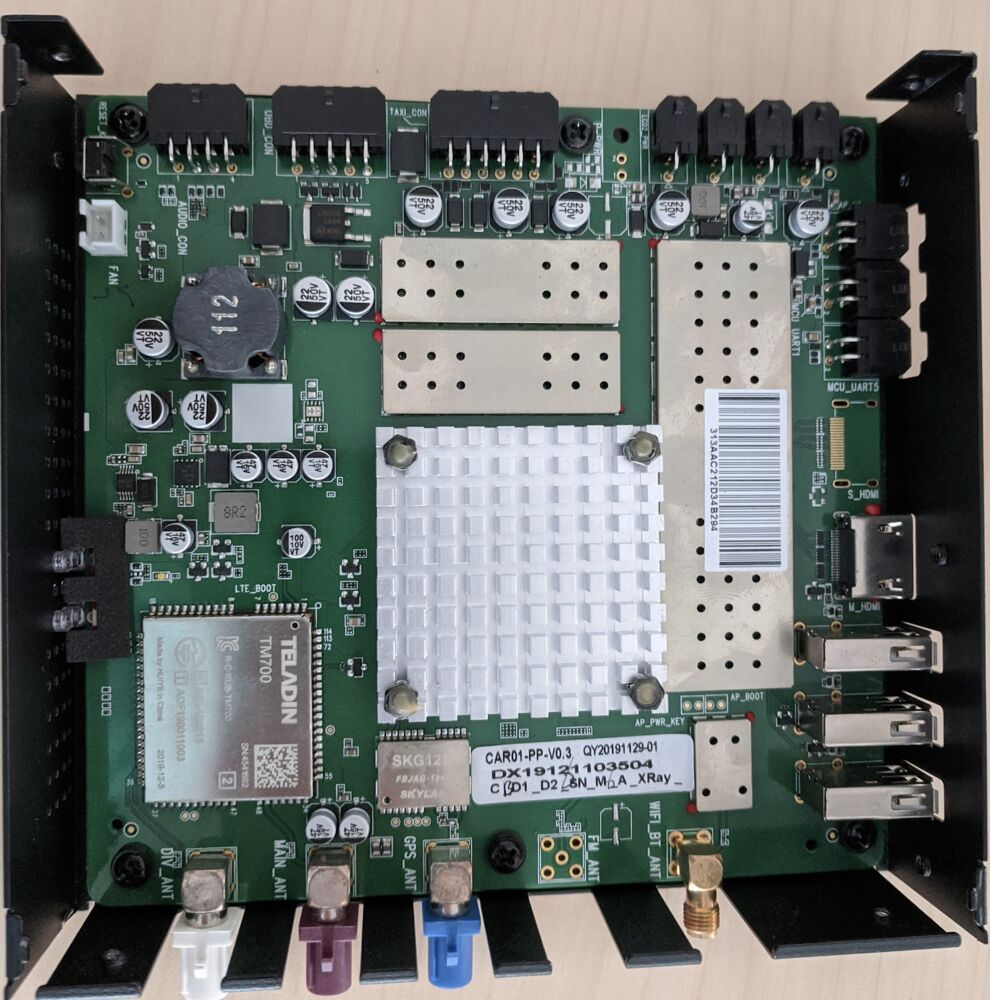
\includegraphics[width=1.9in]{image6.jpg}\hspace{0.2in}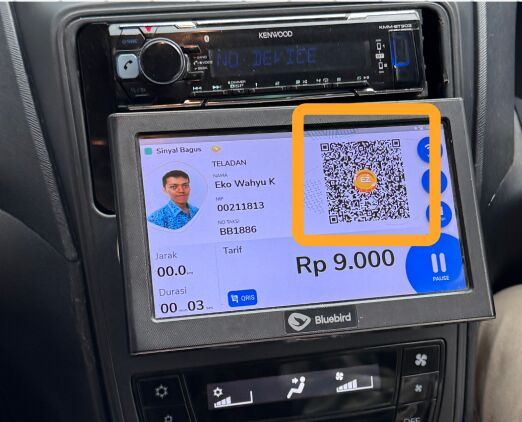
\includegraphics[width=2.2in]{image2.jpg}
\end{center}

\vspace{6pt}

%%%%%%%%%%%%%%%%%%%%%%%%%%%%%%%%%%%%%%%%%%%%%%%%%%%%%%%%%%%%
\resheading{7. Wearable Sprint Tracker (SoleMetrix, Singapore)}
%%%%%%%%%%%%%%%%%%%%%%%%%%%%%%%%%%%%%%%%%%%%%%%%%%%%%%%%%%%%
Designed the end-to-end embedded architecture (Zephyr RTOS) for a sports-technology wearable, including a custom Ultra-Wideband (UWB) ranging protocol achieving 5cm positioning precision for tracking sprint speed and movement on the field. Defined the BLE peripheral API and device driver architecture, plus an efficient sensor-data compression scheme for high-frequency streaming to the host application.
\begin{center}
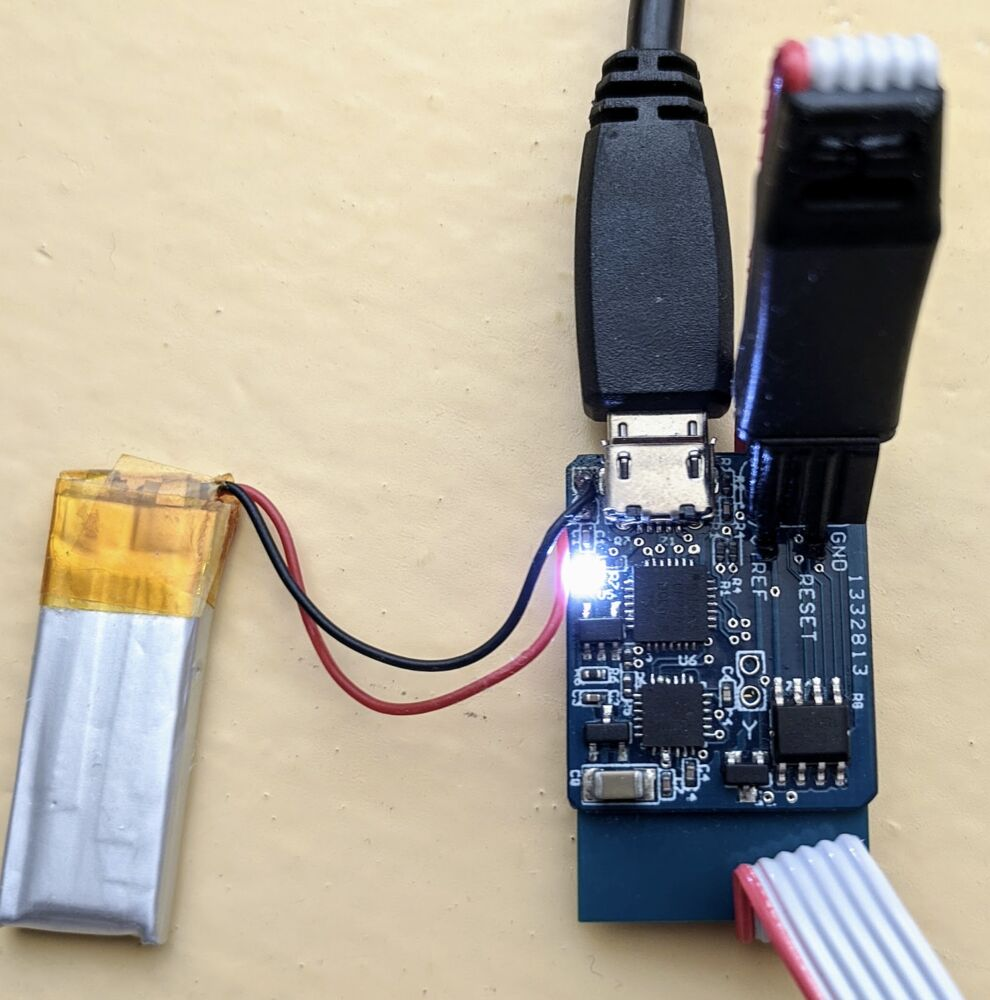
\includegraphics[width=2.0in]{image8.jpg}\hspace{0.2in}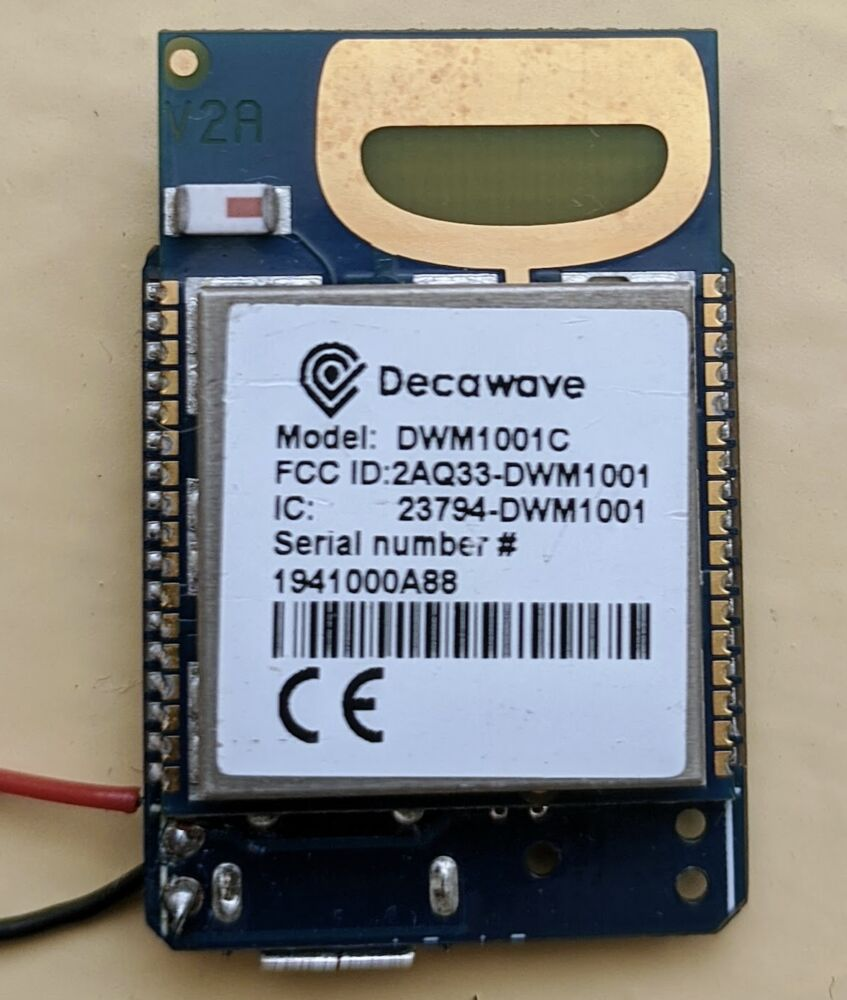
\includegraphics[width=1.7in]{image5.jpg}
\end{center}

\vspace{6pt}

\pagebreak

%%%%%%%%%%%%%%%%%%%%%%%%%%%%%%%%%%%%%%%%%%%%%%%%%%%%%%%%%%%%
\resheading{8. Edge-AI Inference Engine (Nodeflux, Indonesia)}
%%%%%%%%%%%%%%%%%%%%%%%%%%%%%%%%%%%%%%%%%%%%%%%%%%%%%%%%%%%%
Architected the embedded Linux platform (Yocto-based) powering Nodeflux's edge-AI computing devices, including the OTA update strategy and remote-management design. Enabled CPU/GPU-accelerated machine learning inference at the edge for real-time video analytics, deployed in production across a fleet of edge devices.
\begin{center}
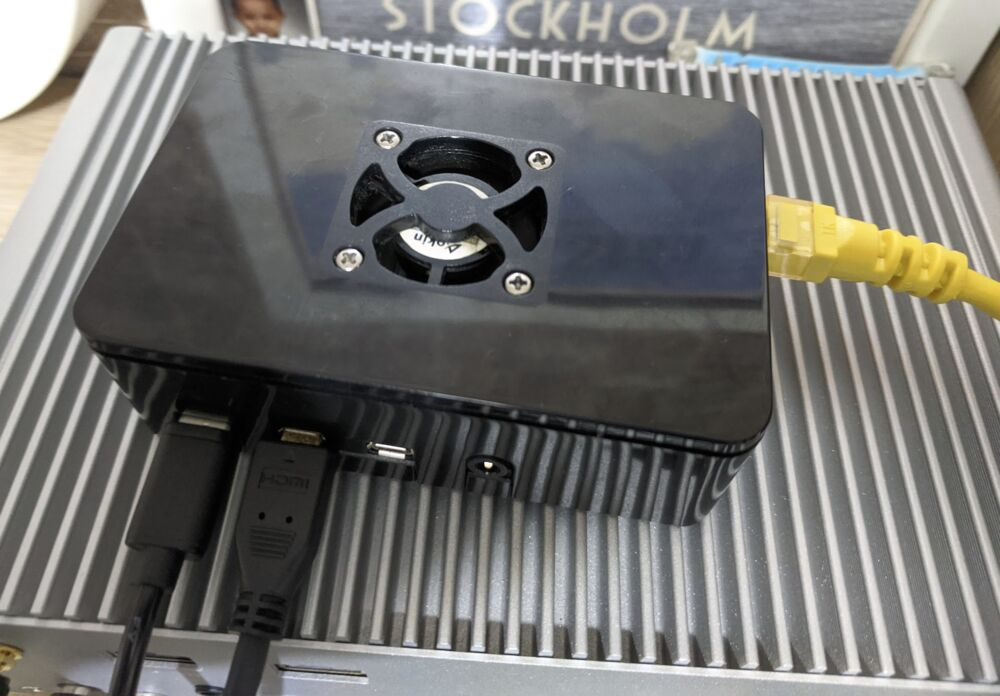
\includegraphics[width=2.3in]{image9.jpg}\hspace{0.2in}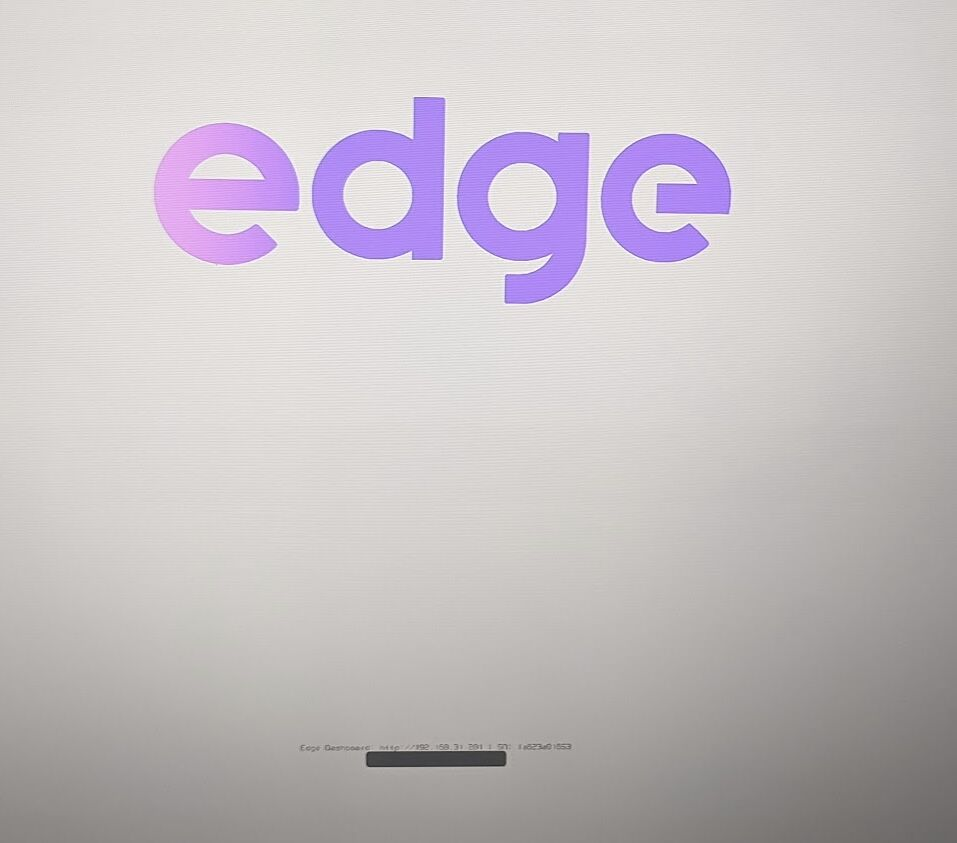
\includegraphics[width=2.0in]{image3.jpg}
\end{center}

\end{document}
